\chapter{Introdução}

Este capítulo apresenta a motivação para o trabalho proposto, os objetivos gerais e secundários, e uma apresentação da estrutura geral do trabalho.

\section{Motivação}

Foguetes de sondagem atmosférica são veículos aeroespaciais sub-orbitais utilizados para levar sensores e experimentos científicos a altos níveis atmosféricos, com o intuito de realizar estudos e análises relacionados às diversas condições ali presentes \cite{isro}.
Estes veículos geralmente utilizam motor de propelente sólido, de um ou dois estágios, e são equipados com sistemas de controle, telemetria e recuperação, além de transportarem o experimento científico, denominado carga-paga \cite{esa, sabbatini2014esa}.
Algumas das vantagens desses veículos são o baixo custo e a menor necessidade de alcance para sistemas de telemetria e rastreio, tendo em vista que não entram em órbita \cite{nasa}.

No contexto de foguetes de sondagem, existem competições que fomentam o desenvolvimento e a competitividade em equipes universitárias de foguetemodelismo \cite{esra}.
Algumas dessas competições tem grande parte de suas categorias definidas nas bases de foguetes de sondagem, com apogeu de voo entre \SI{1}{\kilo\metre} e \SI{10}{\kilo\metre} de altura acima do nível do solo.
Nestes casos, a sequência de operações normal do foguete, simplificada na \autoref{fig:conops}, consiste em: ignição do primeiro estágio do motor, decolagem, período propulsionado, término de queima do primeiro estágio, desacoplamento do primeiro estágio, ignição do segundo estágio, segundo período propulsionado, término de queima do segundo estágio, início do período inercial balístico, apogeu, detecção do apogeu pelos sistemas embarcados, liberação do paraquedas piloto, fase de desaceleração do paraquedas piloto, liberação do paraquedas principal a certa altitude, fase de desaceleração do paraquedas principal e finalmente o pouso \cite{esa, sabbatini2014esa}.
Desacoplamento do primeiro estágio, ignição e fase propulsionada do segundo somente se aplicam a foguetes de dois estágios.

\begin{figure}[htbp]
    \centering
    \caption{Sequência operações simplificada para foguete de sondagem.}
    % % \begin{center}
\begin{tikzpicture}

    % Variables


    \coordinate (bottomleft) at (-0.5,-0.5);
    \coordinate (topright) at (10.5,5);

    \def\coordref[#1](#2){%

        \coordinate(sysref) at (#2);

        \draw[#1, -latex] (sysref) ++(-0.4,-0.3) -- ++(0.9,0) node[midway, below]{$x$};
        \draw[#1, -latex] (sysref) ++(-0.3,-0.4) -- ++(0,0.9) node[midway, left]{$y$};
        \draw[#1, -latex] \centerarc(sysref)(-90:180:0.25);
        \draw[#1] (sysref) node{$+$}
    }

    % \draw[Red,dashed] (bottomleft) rectangle (topright);
    \clip (bottomleft) rectangle (topright);

    \coordinate (O) at (0,0);

    % \draw [help lines, dashed] (bottomleft) grid (topright); % desenha grid
    % \draw [red] (O) node[draw,cross out] {}; % marca pont(0,0)

    % \draw[Red] (4,2)
    %     node[draw, thick, shape=foguete, fill=cmyk_R!25, scale=4] {}
    %     node[draw, circle, inner sep=2pt] {}
    % ;

    % \shade[inner color=yellow,outer color=white] (6,0) rectangle +(2,1);

    % \draw
    %     (-0.5,0) -- (10.5,0)
    % ;


    \coordinate (left) at (-0.5,0);
    \coordinate (right) at (10.5,0);
    \coordinate (middle) at ($(left)!0.5!(right)$);
    \draw[thin, Black!50, path fading=west] (left) -- (middle);
    \draw[thin, Black!50, path fading=east] (middle) -- (right);
    % \shade[draw, inner color=Green!10,outer color=Red] (-0.5,0) -- (10.5,3);


    \draw[cmyk_K] (0,0) node[draw, shape=foguete, fill=cmyk_R, anchor=south, rotate=0] {};

    \draw[cmyk_K] (0.5,2) node[OrangeRed, rotate=170, anchor=south, inner sep=-2.5pt, xshift=0.25pt] {\Fire} node[draw, shape=foguete, fill=cmyk_R, anchor=south, rotate=-10] {};

    \draw[cmyk_K] (5,4) node[draw, shape=foguete, fill=cmyk_R, anchor=south, rotate=-95] {};

    \draw[cmyk_K] (9,0) node[draw, shape=foguete, fill=cmyk_R, anchor=east, rotate=-90] {};



    \begin{pgfonlayer}{background}    % select the background layer
        \clip (bottomleft) rectangle (10.5,0);
        \shade[inner color=SaddleBrown!50,outer color=White] (bottomleft) rectangle (10.5,0.5);
    \end{pgfonlayer}


\end{tikzpicture}
% \end{center}
    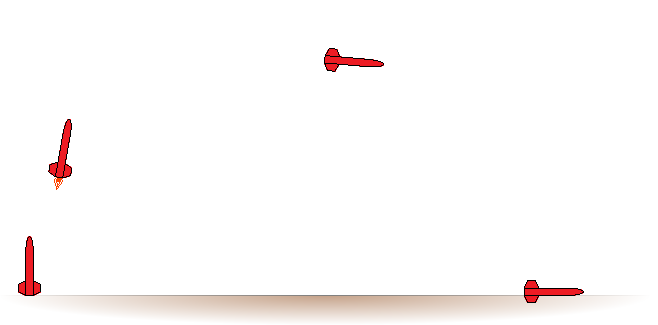
\includegraphics{../pictures/conops}
    \caption*{Fonte: Autor}
    \label{fig:conops}
\end{figure}

A partir do momento do pouso, o próximo objetivo nessas competições consiste em localizar o foguete, vários métodos podem ser empregados nessa situação, desde cores chamativas no veículo e paraquedas, até sinais sonoros.
Essas competições geralmente recomendam, e até exigem, a presença de um \ac{GNSS}, capaz de transmitir as coordenadas do veículo após o pouso para localização, como um \ac{GPS} \cite{irec}.

O processo de localização baseada em dados simples de \ac{GNSS}, latitude e longitude, pode se tornar mais complicado se o grupo de busca não tem certeza de como encontrar essas coordenadas.
Existem dispositivos de \ac{GNSS} portáteis, porém estes podem criar dificuldades na interface com os dados recebidos da telemetria do foguete.
Neste caso, seria possível desenvolver um dispositivo capaz de lidar diretamente com as informações de localização fornecidas pela telemetria e guiar o grupo de busca na direção correta.

Os dados recebidos da telemetria ainda precisam de certo grau de confiabilidade para que sejam devidamente processados e tratados, o que pode ser um problema se o veículo estiver longe do grupo de busca ou o dispositivo de \ac{GNSS} a bordo não esteja apto a fornecer dados corretamente.
Nesse caso, ainda é possível buscar o foguete utilizando o próprio sinal da telemetria, independente dos dados transmitidos.

\section{Objetivos}

O principal objetivo deste trabalho é desenvolver e projetar um dispositivo portátil capaz de indicar a direção da origem de um sinal de \ac{RF} baseado em métodos de detecção de \ac{AoA}.

Como objetivo secundário, a análise comparativa com um sistema de utilidade semelhante, porém baseado inteiramente em coordenadas de \ac{GNSS}.

\section{Estrutura do documento}


O trabalho proposto está organizado em cinco capítulos, apresentando, após este introdutório, mais quatro capítulos.
O \autoref{cap:revbib} traz um levantamento bibliográfico, contendo fundamentação teórica e revisão de trabalhos relacionados.
O \autoref{cap:metodologia} apresenta o detalhe da metodologia adotada na construção do trabalho.
No \autoref{cap:resultados} são apresentados detalhes sobre a performance da simulações realizadas e problemas encontrados.
Por fim, o \autoref{cap:conclusao} traz as considerações finais, conclusões e sugestões para trabalhos futuros que podem resultar em melhorias na presente proposta.

O documento também conta com o \autoref{apdx:codigo}, que apresenta o conjunto de códigos construídos ao longo do desenvolvimento do trabalho.

